\documentclass[12pt, specialist, subf, substylefile = spbu.rtx]{disser}
\usepackage[a4paper, includefoot,
            left=3cm, right=1.5cm,
            top=2cm, bottom=2cm,
            headsep=1cm, footskip=1cm]{geometry}
\usepackage[utf8]{inputenc}
\usepackage[T1, T2A]{fontenc}
\usepackage[english, russian]{babel}
\usepackage{moreverb}
\usepackage{array}
\usepackage{hyperref}
\usepackage{amsthm}

\makeatletter
\newcommand{\@chapapp}{\relax}
\makeatother

\usepackage[title,toc,titletoc,header]{appendix}
\setcounter{tocdepth}{2}
\graphicspath{{diploma3_fig/}}
\newtheorem{theorem}{Теорема}
\newtheorem{definition}{Определение}
\newtheorem{algo}{Алгоритм}
\newcommand{\Expect}{\mathsf{E}}
\newcommand{\CVaR}{\mathsf{CVaR}}
\newcommand{\Var}{\mathsf{Var}}
\DeclareGraphicsExtensions{.pdf,.png}
\DeclareMathOperator*{\toplim}{\overline\lim}
\DeclareMathOperator*{\botlim}{\underline\lim}
\DeclareMathOperator*{\tou}{\longrightarrow}
\newcommand{\MDA}{\mathsf{MDA}}
\begin{document}

Бутстрап.
  
Вот то, что я у вас беру за основу:

Бутстрап-оценка, задача:

$$
\hat{\omega}_n = W^*_n = \hat{P}_n\big( T(P^*_n)-T(\hat{P}_n) > a_n \big),
$$
где $P^*_n$ -- эмпирическая мера $X^*_i \sim \hat{P_n}$.

Оцениваем $W^*_n$:
\begin{equation}\label{eq:w1}
\hat{W}_n = \frac{1}{n} \sum_{i=1}^k \chi\big( T(P^*_{ni})-T(\hat{P}_n) > a_n\big).
\end{equation}

Взвешенный бутстрап:

$$
\tilde{P}_n (Y=X_i) = \frac{1}{n}(1+a_n(h_n(X_i)-\bar{h}_n)),
$$
$$
h = q \sigma_q^{-2}, q\text{ -- функця влияния $T(P)$.}
$$


Дальше мои попытки: $b_n=a_n \sigma$, 
$$
h_n(X_i)-\bar{h}_n = h(X_i),
$$
тогда оценка получается
$$
\tilde{P}_n (Y=X_i) = \frac{1}{n}(1+b_n \frac{h(X_i)}{\sigma}).
$$
Для начала генерируется некоторое (большое) количество $X_i \sim exp(\alpha)$ для модифицированной оценки Хилла 

\begin{equation}\label{eq:w2}
T(P)=\hat{\alpha}_H^{-1}=\frac{1}{n-m+1} \sum\limits_{i=m}^n Y_{i:n}- Y_{m:n}.
\end{equation}

Строится дискретное распределение $\tilde{P}_n (x=X_i)$ с учетом функции влияния. Далее для выборки равномерно генерируется $n$ вероятностей $p_n \in [0;1]$, и для них моделируется соответствующая бутстрап-выборка. Бутстрап получается, заметно хуже, чем все остальное, но получается (рисунок~\ref{ris:plot_boots}). 

\begin{figure}[!!h]
\center{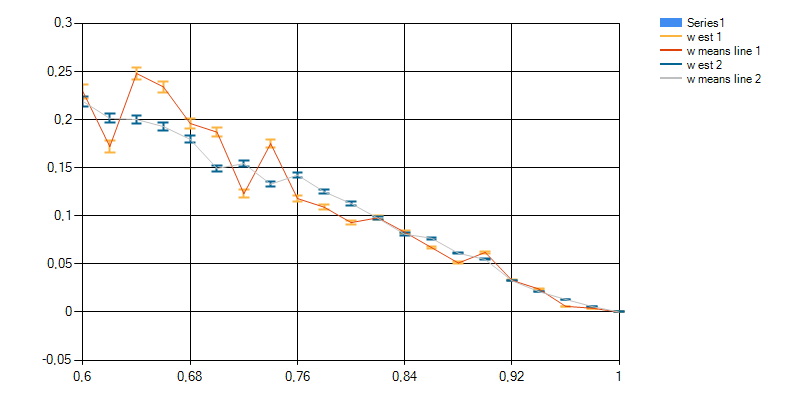
\includegraphics[width=1\linewidth]{plot_boots}}
\caption{Бутстрап. Синий: оценка сущ. выборки, оранжевый бутстрап}
\label{ris:plot_boots}
\end{figure}


Почему-то не получается оценка <<в лоб>>, когда я просто беру $X_i \sim exp(\alpha)$, подставляю в~\eqref{eq:w2} и считаю как доверительный интервал. Если я беру границу $b_n$, он получается выше, чем линия оценки существенной выборки (рисунок~\ref{ris:plot_bn}). Если $a_n$, то получается рисунок~\ref{ris:plot_an}.


\begin{figure}[!!h]
\center{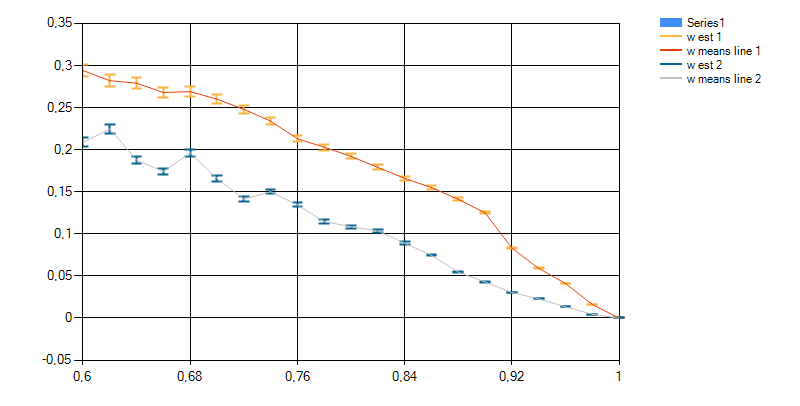
\includegraphics[width=1\linewidth]{plot_bn}}
\caption{bn. Синий: оценка сущ. выборки, оранжевый оценка <<в лоб>>}
\label{ris:plot_bn}
\end{figure}


\begin{figure}[!!h]
\center{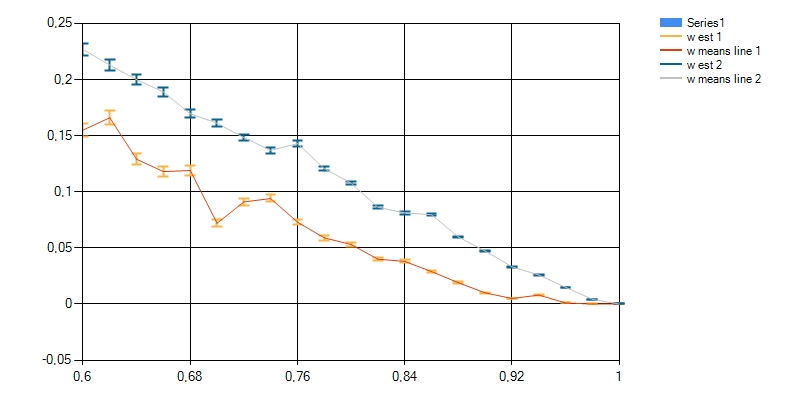
\includegraphics[width=1\linewidth]{plot_an}}
\caption{an. Синий: оценка сущ. выборки, оранжевый оценка <<в лоб>>}
\label{ris:plot_an}
\end{figure}

Разница между этими двумя вариантами в том, что я в первом случае использую индикатор 
$$
\chi \big( T(P^*_n)-T(\hat{P}_n) > b_n \big)
$$
а во втором случае 
$$
\chi \big( T(P^*_n)-T(\hat{P}_n) > b_n \sigma_q \big)
$$

Третий случай работает, но мне кажется, это какая-то чушь (рисунок~\ref{ris:plot_cn}.):
$$
\chi \big( T(P^*_n)-T(\hat{P}_n) > b_n \sqrt{\sigma_q} \big)
$$

\begin{figure}[!h]
\center{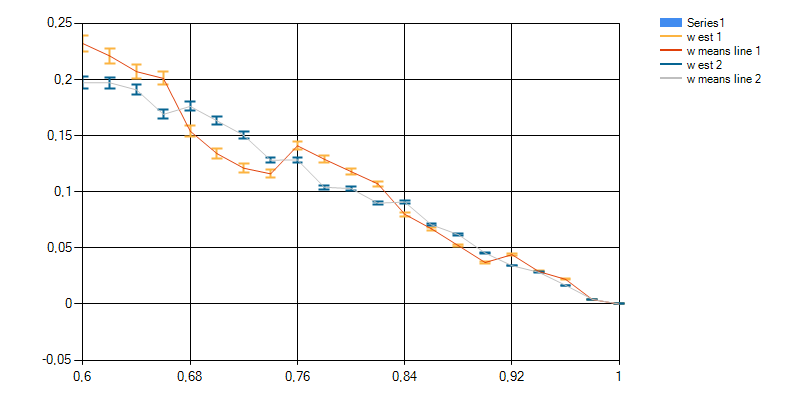
\includegraphics[width=1\linewidth]{plot_cn}}
\caption{Третий случай. Синий: оценка сущ. выборки, оранжевый оценка <<в лоб>>}
\label{ris:plot_cn}
\end{figure}




















\end{document}